\documentclass{optica-article}

\journal{opticajournal}
\articletype{Research Article}

\usepackage{lineno}
\linenumbers

\newcommand{\chitwo}{\chi^{(2)}}
\newcommand{\chithree}{\chi^{(3)}}
\newcommand{\chicasc}{\chi^{(3)}_{\mathrm{casc}}}
\newcommand{\chinat}{\chi^{(3)}_{\mathrm{nat}}}
\newcommand{\Dom}{\Delta\omega}
\newcommand{\etag}{\eta_{\mathrm{geom}}}
\newcommand{\f}{\mathbf f}

% placeholder for figures that are not yet drawn
\newcommand{\figbox}[1]{%
  \fbox{\parbox[c][#1][c]{0.9\linewidth}{\centering\small figure in preparation}}}

\begin{document}

\title{Resonant cascaded Kerr nonlinearity in $\chi^{(2)}$ metasurfaces}

% please discuss the authors' order with Andrea and Jacob
\author{Nikita Nefedkin,\authormark{1,*} Sedigheh Esfahani,\authormark{1} Jacob B. Khurgin,\authormark{2} and Andrea Al\`u\authormark{1}}

\address{\authormark{1}Photonics Initiative, Advanced Science Research Center, City University of New York, New York, New York 10031, USA\\
\authormark{2}Department of Electrical and Computer Engineering, Johns Hopkins University, Baltimore, Maryland 21218, USA}

\email{\authormark{*}nnefedkin@gc.cuny.edu}

\begin{abstract*}
A detuned second-harmonic resonance can replace the phase mismatch that
sets the cascaded Kerr nonlinearity of bulk crystals.  We derive the
cascaded susceptibility of a general resonator, with an overlap bounded by
one and the bulk result as a limit.  Its sign follows the detuning $\Dom$,
it carries a nonlinear loss, and its product with the bandwidth does not
depend on the quality factor.  In doubly resonant LiNbO$_3$ metasurfaces
with a second-harmonic quality factor of 4000 it is about 20 times the
native Kerr response, and in poled microrings 400 to 3000 times.  For a
singly resonant metasurface we propose a picosecond Z-scan that isolates
the part of the response odd in $\Dom$.
\end{abstract*}


\section{Introduction}

\begin{enumerate}
\item Kerr nonlinearity underlies all-optical switching, optical
  bistability, parametric oscillation and frequency combs.  The native
  $\chithree$ of low-loss dielectrics is small, about
  $3\times10^{-21}$~m$^2$/V$^2$ in LiNbO$_3$ (Supplement 1, Section 5), and
  its sign is set by the material.  Field enhancement in resonant
  nanostructures increases the nonlinear phase per unit power without
  changing either~\cite{khurgin2013}.
\item Two cascaded second-order processes act on the pump as a Kerr
  medium.  The effect was predicted by Ostrovskii~\cite{ostrovskii1967},
  observed in KTP as a nonlinear refraction that changes sign with the
  phase mismatch~\cite{desalvo1992}, reviewed in Ref.~\cite{stegeman1996}
  and described microscopically as a collective effect~\cite{khurgin1997}.  In bulk crystals its
  strength scales as $1/\Delta k$, with $\Delta k$ the phase mismatch, and
  it is used for soliton compression~\cite{bache2007josab,bache2010,zhou2012}.
  Khurgin and co-workers proposed a second-harmonic resonance in place of
  $\Delta k$ for surface-emitting structures~\cite{khurgin1994,lee1995},
  with an enhancement over the native response of the order of the quality
  factor of that resonance~\cite{khurgin1997}.
\item In $\chitwo$ cavities the eliminated second harmonic acts on the pump
  as a Kerr term with a nonlinear
  loss~\cite{drummond1980,majumdar2013,fryett2015,gustin2025}.  In a
  LiNbO$_3$ microdisk and in AlN microrings this term produced four-wave
  mixing~\cite{liu2019ol,cui2022}, and in an AlN microring the
  detuning of the second-harmonic mode tuned the self-phase modulation from
  $-2.7$ to $+4.7$ times its native value~\cite{cui2025}.  In
  free-space cavities around periodically poled LiNbO$_3$ crystals, an
  effective Kerr response estimated at $10^2$ to above $10^3$ times the
  native one drives dissipative quadratic
  solitons~\cite{nie2026,musgrave2026,musgrave2026opo}.  Four-wave
  mixing in a poled thin-film waveguide corresponds to an effective Kerr
  index $1.6\times10^4$ times the native value~\cite{li2026}.  In nanoresonators
  and metasurfaces, quasi-bound states in the continuum enhance
  second-harmonic generation~\cite{carletti2018,koshelev2020,vabishchevich2018,liu2019,anthur2020},
  also in LiNbO$_3$~\cite{fedotova2020}, and cascaded second-order processes
  have produced third-harmonic light~\cite{celebrano2019,gennaro2022}.  The
  back-conversion of the second harmonic in a metasurface has been treated
  as pump depletion~\cite{tu2024}; to our knowledge, the Kerr response it
  produces on the pump has not been evaluated or compared with the native
  response of the host.
\item We extend the resonant replacement of $\Delta k$ to a general
  resonator with vector modes.  The cascaded susceptibility takes one closed
  form with a geometric overlap $\etag\le1$.  It scales as
  $\omega_1/\Dom$, that is as the quality factor $Q_2$ of the
  second-harmonic mode at a fixed ratio of $\Dom$ to its linewidth, and
  changes sign with $\Dom$ [Fig.~\ref{fig:concept}(a)].  For any resonator,
  the product of strength and bandwidth depends on neither $Q_2$ nor
  $\Dom$, and the ratio $R$ of the cascaded to the native Kerr response of
  the same mode depends on the host through a single figure of merit.  In
  LiNbO$_3$, $R$ is about 20 in a doubly resonant metasurface with $Q_2=4000$
  and $\etag=0.3$, with a bandwidth of 0.1~THz, and 400 to 3000 in poled
  microrings, with bandwidths below 1~GHz.  In a microring the cascaded
  shift follows from the measured second-harmonic efficiency, so the
  formula can be tested with no free parameter.  For a singly resonant
  metasurface, where the native response does not vary across the
  second-harmonic resonance, we propose a picosecond Z-scan that isolates the
  part of the response odd in $\Dom$.
\end{enumerate}

\begin{figure}[htbp]
  \centering
  \figbox{4.5cm}
  \caption{Cascaded Kerr response at a second-harmonic resonance.
    (a)~Second-harmonic generation and difference-frequency generation
    through a mode at $\omega_2$, detuned by $\Dom=2\omega_1-\omega_2$.
    (b)~Doubly resonant LiNbO$_3$ metasurface with a quasi-bound state at
    $\omega_1$ and a symmetry-protected mode near $2\omega_1$ in one
    meta-atom.
    (c)~Periodically poled microring with pump and second-harmonic modes.
    (d)~Real (solid) and imaginary (dashed) parts of $\chicasc$ versus
    $\Dom$ in units of the second-harmonic linewidth $\gamma_2$, normalised to
    $|\mathrm{Re}\,\chicasc|$ at $\Dom=2\gamma_2$.}
  \label{fig:concept}
\end{figure}


\section{Cascaded susceptibility at a second-harmonic resonance}\label{sec:theory}

A pump at frequency $\omega_1$ excites a mode $\f_1$ of the structure, with
resonance frequency $\omega_a$ and energy decay rate
$\gamma_1=\omega_a/Q_1$, and its second harmonic falls near a mode $\f_2$
with frequency $\omega_2$ and decay rate
$\gamma_2=\omega_2/Q_2\simeq2\omega_1/Q_2$.  Real fields are written as
$\mathbf E e^{-i\omega t}+\mathrm{c.c.}$, so that with $\mathbf E_1$ and
$\mathbf E_2$ the complex amplitudes at $\omega_1$ and $2\omega_1$ the
second-harmonic, difference-frequency and self-phase-modulation
polarisations are
$\varepsilon_0\chitwo\mathbf E_1\mathbf E_1$,
$2\varepsilon_0\chitwo\mathbf E_2\mathbf E_1^*$ and
$3\varepsilon_0\chithree|\mathbf E_1|^2\mathbf E_1$~\cite{boyd2020}.
Under Kleinman symmetry one tensor $\chitwo_{ijk}(\mathbf r)$ describes both
second-order processes.  For the field
$a_1\f_1e^{-i\omega_1t}+a_2\f_2e^{-2i\omega_1t}+\mathrm{c.c.}$, mode $n$
stores the energy $2N_n|a_n|^2$, with
$N_n=\tfrac12\int(\varepsilon_0\tilde\varepsilon_n|\f_n|^2+\mu_0|\mathbf h_n|^2)\,d^3r$,
$\mathbf h_n$ the magnetic profile and
$\tilde\varepsilon_n=\partial(\omega\varepsilon_r)/\partial\omega$ at the
resonance frequency of mode $n$.  Projecting Maxwell's equations onto the two modes for slowly
varying amplitudes~\cite{johnson2002,rodriguez2007} gives
\begin{align}
  \dot a_1&=\bigl(i\delta_1-\tfrac{\gamma_1}{2}\bigr)a_1
    +i\beta_1^*a_1^*a_2+i\alpha_3|a_1|^2a_1+\sqrt{\gamma_1^{\mathrm e}/2N_1}\,s,\label{eq:cmt1}\\
  \dot a_2&=\bigl(i\Dom-\tfrac{\gamma_2}{2}\bigr)a_2+i\beta a_1^2,\label{eq:cmt2}
\end{align}
with the pump detuning $\delta_1=\omega_1-\omega_a$, the second-harmonic
detuning $\Dom=2\omega_1-\omega_2$, and $\gamma_1^{\mathrm e}$ the decay
rate into the channel of an incident wave of power $|s|^2$.  The couplings are
$\beta=\varepsilon_0\omega_1M/N_2$ and $\beta_1=\varepsilon_0\omega_1M/N_1$,
with the overlap $M=\int\chitwo_{ijk}f^*_{2,i}f_{1,j}f_{1,k}\,d^3r$, and
the native Kerr coefficient is
$\alpha_3=(3\varepsilon_0\omega_1/2N_1)\int\chithree_{ijkl}f^*_{1,i}f_{1,j}f_{1,k}f^*_{1,l}\,d^3r$.
The factor 2 of difference-frequency generation makes
$N_1\beta_1=N_2\beta$, so that the energy
$2(N_1|a_1|^2+N_2|a_2|^2)$ is conserved in the absence of loss and drive
(Supplement 1, Section 1).

When the pump envelope varies slowly on the time scale
$|\Dom+i\gamma_2/2|^{-1}$, Eq.~\eqref{eq:cmt2} gives
$a_2=-\beta a_1^2/(\Dom+i\gamma_2/2)$.  Inserted into
Eq.~\eqref{eq:cmt1}, this adds the term
$i\alpha_{\mathrm{casc}}|a_1|^2a_1$ with
$\alpha_{\mathrm{casc}}=-\beta_1^*\beta/(\Dom+i\gamma_2/2)$, which has the
form of the native Kerr term.  Writing
$\alpha_3=(3\varepsilon_0\omega_1/2N_1)\chinat\int_{\mathrm{NL}}|\f_1|^4d^3r$
defines the native susceptibility $\chinat$ of the second-order material,
where $\int_{\mathrm{NL}}$ extends over that material, and the analogous
relation between $\alpha_{\mathrm{casc}}$ and $\chicasc$ defines the
cascaded susceptibility,
\begin{equation}
  \chicasc=-\frac{2\varepsilon_0\omega_1}{3N_2}\,
    \frac{|M|^2}{(\Dom+i\gamma_2/2)\int_{\mathrm{NL}}|\f_1|^4d^3r}
  =-\frac{2\omega_1|\chitwo|^2\etag}{3n_2^2\,(\Dom+i\gamma_2/2)} ,
  \label{eq:chi3casc}
\end{equation}
where $n_2$ is the smallest principal refractive index of the
second-order material at $2\omega_1$, $|\chitwo|$ is the largest value of
$|\chitwo_{ijk}u^*_iv_jv_k|$ over unit vectors ($2d_{33}$ for LiNbO$_3$;
Supplement 1, Section 1), and
\begin{equation}
  \etag=\frac{\varepsilon_0n_2^2\,|M|^2}{|\chitwo|^2N_2\int_{\mathrm{NL}}|\f_1|^4d^3r}\le1
  \label{eq:eta}
\end{equation}
is a geometric overlap that does not depend on the normalisation of the
modes.  The bound follows from the Cauchy--Schwarz inequality for modes
with normal dispersion (Supplement 1, Section 1).  The real part of
$\chicasc$ is odd in $\Dom$; for $\Dom>0$ it is negative and shifts the
pump resonance to higher frequency [Fig.~\ref{fig:concept}(d)].  The
imaginary part is even in $\Dom$ and positive, and describes an
intensity-dependent loss of pump power into the second-harmonic mode, the
cascaded analogue of two-photon absorption~\cite{gustin2025}.

Equation~\eqref{eq:chi3casc} also follows without a coupled-mode equation
for the second harmonic.  Its field is the Green's function of the
structure at $2\omega_1$ integrated against the source
$\varepsilon_0\chitwo\mathbf E_1\mathbf E_1$, and inserting it into the
difference-frequency polarisation gives a cascaded polarisation with the
nonlocal kernel $\chitwo(\mathbf r)G(\mathbf r,\mathbf r';2\omega_1)\chitwo(\mathbf r')$.
Near an isolated mode the pole term of
$G$~\cite{sauvan2013,lalanne2018} factorises the kernel into the overlaps
$M$ and $M^*$, and projection onto $\f_1$ returns
Eq.~\eqref{eq:chi3casc} (Supplement 1, Section 2).

For a uniform medium with refractive indices $n_1$ and $n_2$ at
$\omega_1$ and $2\omega_1$ (isotropic, or with fields along the axis of
smallest index) filling a periodic box, the pump mode at
wavevector $k_1$ couples only to the second-harmonic mode at $2k_1$.  When
dispersion within the second-harmonic band is neglected, its frequency is
$\omega_2=2\omega_1n_1/n_2$ and $\etag=1$ for aligned polarisations.
Equation~\eqref{eq:chi3casc} then becomes $-2|\chitwo|^2/[3(n_2^2-n_1^2)]$
to first order in $n_2-n_1$.  This is the susceptibility carried by the
bound second-harmonic wave of a bulk crystal, which for
$\Delta k=2\omega_1(n_2-n_1)/c$ equals the bulk result
$-2\omega_1|\chitwo|^2/(3cn_2\Delta k)$~\cite{desalvo1992,stegeman1996}
(Supplement 1, Section 3).  A resonator thus replaces the material
mismatch $c\Delta k/n_2$, $0.04\,\omega_1$ in LiNbO$_3$, by $\Dom$,
$10^{-3}\omega_1$ for $Q_2=4000$ and $\Dom=2\gamma_2$; $\etag$
is the fraction of the bound-wave coupling that the two modes retain.

Equation~\eqref{eq:chi3casc} assumes a single second-harmonic mode, a
stable steady state and a slowly varying pump envelope.  Equations
\eqref{eq:cmt1} and \eqref{eq:cmt2} omit the native self- and cross-phase
modulation that involve the second-harmonic mode.  For comparable overlaps
these stay small as long as the cascaded shift of the pump resonance is small
compared with both $|\Dom|R/4$ and $|\Dom|(R/2)^{1/2}$, with $R$ of
Eq.~\eqref{eq:R} (Supplement 1, Section 4).  Other second-harmonic modes, cascaded optical rectification
with the electro-optic effect~\cite{bosshard1995} and the longitudinal part
of the bound second harmonic~\cite{kolleck2004} add a background that varies
little with $\Dom$ across the resonance.


\section{Limits and host materials}\label{sec:limits}

The second-harmonic mode sets the response time of the cascade.  A
component of $a_1^2(t)$ at frequency $\Omega$ measured from $2\omega_1$ enters
Eq.~\eqref{eq:cmt1} with the cascaded susceptibility
$-C/(\Dom+\Omega+i\gamma_2/2)$, where
$C=2\omega_1|\chitwo|^2\etag/(3n_2^2)$ (Supplement 1, Section 4).  This
response has a single pole at $\Omega=-\Dom-i\gamma_2/2$ and is
quasi-static for modulation frequencies small compared with
$|\Dom+i\gamma_2/2|$.  At $\Dom=2\gamma_2$ it stays between 0.81 and 1.30 of
its static value over a band of full width $\gamma_2/2\pi$, which is 0.1~THz for
$Q_2=4000$ at a pump wavelength of 1.55~\textmu m.  The static value obeys
$|\chicasc|\,|\Dom+i\gamma_2/2|=C$ for any $Q_2$ and $\Dom$, so raising $Q_2$
at fixed $\Dom/\gamma_2$ increases $|\chicasc|$ and lowers its bandwidth
$\Delta f$ in the same proportion.  For any modulation band narrower than
the distance of the pole from the origin,
$\Delta f\le|\Dom+i\gamma_2/2|/2\pi$, this identity gives
\begin{equation}
  |\chicasc|\,\Delta f\le\frac{\omega_1|\chitwo|^2\etag}{3\pi n_2^2},
  \label{eq:sumrule}
\end{equation}
whose right-hand side depends on neither $Q_2$ nor $\Dom$
[Fig.~\ref{fig:limits}(a)].  The pole also gives the sum rule
$\int\mathrm{Im}\,\chicasc(\Omega)\,d\Omega=\pi C$ over the modulation
frequency, so the integrated nonlinear absorption does not depend on the
linewidth.  Trade-offs between the
strength and the bandwidth of resonantly enhanced nonlinearities have been
discussed for slow-light and resonant nonlinear
devices~\cite{khurgin2005,khurgin2010,khurgin2023} and for harmonic
generation~\cite{shcherbakov2019}, and appear in a cavity-enhanced cascaded
frequency shifter~\cite{gorbounova1996}.

Bulk LiNbO$_3$ at its natural phase mismatch has
$|\chicasc|\approx5\times10^{-21}$~m$^2$/V$^2$.  In bulk crystals the cascaded
response is nonlocal in time on a scale set by the phase and
group-velocity mismatches~\cite{bache2007ol}, and for strong phase
mismatch it is ultrafast and spans an octave~\cite{zhou2012}, so its
bandwidth exceeds 10~THz.  A doubly resonant LiNbO$_3$ metasurface with
$Q_2=4000$ and $\etag=0.3$ reaches about $6\times10^{-20}$~m$^2$/V$^2$
over 0.1~THz.  The product $|\chicasc|\,\Delta f$ of bulk cascading, above
$5\times10^{-8}$~m$^2\,$V$^{-2}\,$Hz, therefore exceeds the bound of
Eq.~\eqref{eq:sumrule} for this metasurface,
$1\times10^{-8}$~m$^2\,$V$^{-2}\,$Hz; the bound itself does not apply to
the bulk response, which has no single pole.  The resonator is preferable
when the nonlinear element must be a sub-micrometre layer or must change
sign over a small detuning.

The cascaded and native Kerr terms act on the same pump mode, so the field
enhancement of the pump resonance cancels in their ratio
$R=|\mathrm{Re}\,\alpha_{\mathrm{casc}}|/\alpha_3=|\mathrm{Re}\,\chicasc|/\chinat$.
At $\Dom=2\gamma_2$,
\begin{equation}
  R\simeq\frac{Q_2\,\etag}{6}\,F,\qquad F=\frac{|\chitwo|^2}{n_2^2\chinat},
  \label{eq:R}
\end{equation}
which neglects $(\gamma_2/2\Dom)^2$ and overestimates $R$ by one part in 16.  The host
enters only through the dimensionless figure of merit $F$.  With the
constants of Supplement 1, Section 5, $F$ is 0.10 for LiNbO$_3$ and between
$2.5\times10^{-3}$ and $4.5\times10^{-3}$ for GaP, AlN and
Al$_{0.2}$Ga$_{0.8}$As, where the GaP value is an upper estimate.  With $\etag=0.3$, $R=1$ is reached at
$Q_2\approx200$ in LiNbO$_3$ and between 4000 and 8000 in
the three semiconductors [Fig.~\ref{fig:limits}(b)].  Estimates of the native
Kerr index of LiNbO$_3$ at 1.55~\textmu m span a factor of 1.8 and those of
$d_{33}$ span 20\%; together they place $R$ at $Q_2=4000$ between 11 and 30.  GaAs is not included because its second
harmonic at 775~nm lies above the band gap.

The imaginary part of Eq.~\eqref{eq:chi3casc} fixes the ratio of nonlinear
loss to nonlinear refraction.  It is
$\rho=|\mathrm{Im}\,\chicasc/\mathrm{Re}\,\chicasc|=\gamma_2/(2|\Dom|)$,
which is $1/4$ at $\Dom=2\gamma_2$.  A Kerr resonator with this loss is
bistable for some pump detuning only if $\rho<1/\sqrt3$, and the same
condition governs parametric gain of a pair of sidebands (Supplement 1,
Section 4).  When the cascaded term dominates, both therefore require
$|\Dom|>\sqrt3\gamma_2/2$; otherwise $\rho$ must be evaluated for the sum of the
cascaded and native terms.  Bistability also needs a pump detuning
$|\delta_1|$ above $\sqrt3\gamma_1/2$ without nonlinear loss and above $1.75\gamma_1$
at $\rho=1/4$.  Because $\Dom$ is defined with the pump frequency, the cold
resonator must then be built with the mismatch
$2\omega_a-\omega_2=\Dom-2\delta_1$.

The second-harmonic mode stores the energy of the pump mode multiplied by
$S/|\Dom|$, where $S=|\mathrm{Re}\,\alpha_{\mathrm{casc}}||a_1|^2$ is the
cascaded shift of the pump resonance.  In a continuous-wave steady state the
elimination of $a_2$ is exact at any power.  The steady state of
Eqs.~\eqref{eq:cmt1} and \eqref{eq:cmt2} can, however, lose stability through
self-pulsing~\cite{drummond1980} once $S/|\Dom|$ exceeds a value between
about 1 and 10 that depends on $\gamma_1$ and $\delta_1$.

\begin{figure}[htbp]
  \centering
  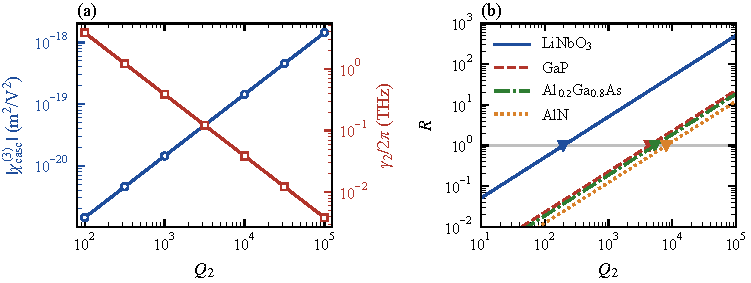
\includegraphics[width=\linewidth]{figures/fig2_limits.pdf}
  \caption{(a)~$|\chicasc|$ of LiNbO$_3$ at $\Dom=2\gamma_2$ (circles, left
    axis) and the bandwidth $\gamma_2/2\pi$ (squares, right axis) versus
    $Q_2$, for $\etag=0.3$ and a pump wavelength of 1.55~\textmu m.
    (b)~$R$ from Eq.~\eqref{eq:R} versus $Q_2$ at $\Dom=2\gamma_2$ and
    $\etag=0.3$ for the hosts of Supplement 1, Section 5 (line styles);
    triangles and the horizontal line mark $R=1$.}
  \label{fig:limits}
\end{figure}


\section{Metasurface implementation}\label{sec:meta}

\subsection{Doubly resonant metasurface}
% FOR THE DESIGN (Sedigheh): first paragraph = unit cell, symmetry of the two
% modes, selection rules for the d33 orientation, how Domega is tuned.

In a doubly resonant metasurface a quasi-bound state at $\omega_1$ couples
the pump from free space~\cite{koshelev2018}, and a symmetry-protected bound
state in the continuum near $2\omega_1$ holds the second harmonic
[Figs.~\ref{fig:concept}(b) and \ref{fig:double}(a)].  Symmetry protects
the latter only while the second harmonic lies below the first diffraction
order of the substrate and the cladding~\cite{hsu2016,cerjan2021}.  For a
pump at 1.55~\textmu m on silica this requires a period below 535~nm, at
which a first-order pump resonance at the $\Gamma$ point of the Brillouin
zone would need an effective
index above 2.9, out of reach in LiNbO$_3$.  The pump mode then has to be
folded to $\Gamma$ by a perturbation that doubles the period, as in
Ref.~\cite{wang2020}, and this perturbation opens weak second-harmonic
diffraction channels; a suspended film raises the limit on the period to
775~nm.  A doubly resonant cavity of this kind was
proposed~\cite{minkov2019} and demonstrated~\cite{wang2020} for
second-harmonic generation.  The overlap $M$ is nonzero only
if the unit-cell symmetry of $\f_2$ matches that of $\chitwo$ contracted
with $\f_1\f_1$, which sets selection rules for the $d_{33}$ orientation of
a LiNbO$_3$ film~\cite{fedotova2020}.  At normal incidence both modes lie
at $\Gamma$, which removes the bulk phase-matching condition.  The mismatch
$\Dom$ can be tuned by temperature or by the electro-optic effect.
Random variations of size and position lower the quality factor of the
second-harmonic mode as the inverse square of their
amplitude~\cite{kuhne2021,maslova2021}, and an array of $N_p$ periods limits
it to a value that grows as $N_p^2$ for a one-dimensional
array~\cite{bulgakov2017}.  The array and the pump spot must therefore span
many periods.  Measured quality factors of such modes are about $10^4$ in
Si$_3$N$_4$ slabs near 740~nm~\cite{hsu2013}, 800 for the second-harmonic
mode of a GaN cavity at 775~nm~\cite{wang2020} and above 8000 in
LiNbO$_3$-on-insulator metasurfaces at 1.55~\textmu m~\cite{difrancescantonio2025};
we have found no report of $Q_2=4000$ at 775~nm in LiNbO$_3$.

For $Q_2=4000$, $\etag=0.3$ and $|\Dom|=2\gamma_2$, Eq.~\eqref{eq:R} gives
$R\approx20$ in LiNbO$_3$ [Fig.~\ref{fig:double}(b)].  For $\Dom<0$ the
cascaded and native terms add: self-phase modulation scales as $1+R$, and
four-wave mixing between sidebands within $|\Dom+i\gamma_2/2|$ of the pump
scales as $(1+R)^2$ [Fig.~\ref{fig:double}(d)].  For $\Dom>0$ they subtract,
and the net Kerr response reverses sign when $R>1$.  The pump energy needed
for a given shift scales as $1/(1+R)$; the second harmonic stores a further
fraction equal to the cascaded shift divided by $|\Dom|$
(Section~\ref{sec:limits}), which is small for a shift of one pump
linewidth when $\gamma_1\ll|\Dom|$ and reaches 0.5 to 0.8 at the folds of
Fig.~\ref{fig:double}(c), where $\gamma_1=\gamma_2$.
The bistability threshold falls by less, by a factor of about $(1+R)/5$ for
$R$ between 10 and 100 at $|\Dom|=2\gamma_2$, because the cascaded loss
raises the pump detuning needed for bistability [Fig.~\ref{fig:double}(c);
Supplement 1, Section 4].  Cascaded bistability
has been observed with a phase-mismatched second harmonic in a monolithic
MgO:LiNbO$_3$ resonator pumped by a continuous-wave laser~\cite{white1996},
and few-photon bistability in doubly resonant $\chitwo$ nanocavities has
been analysed~\cite{fryett2015}.

\begin{figure}[htbp]
  \centering
  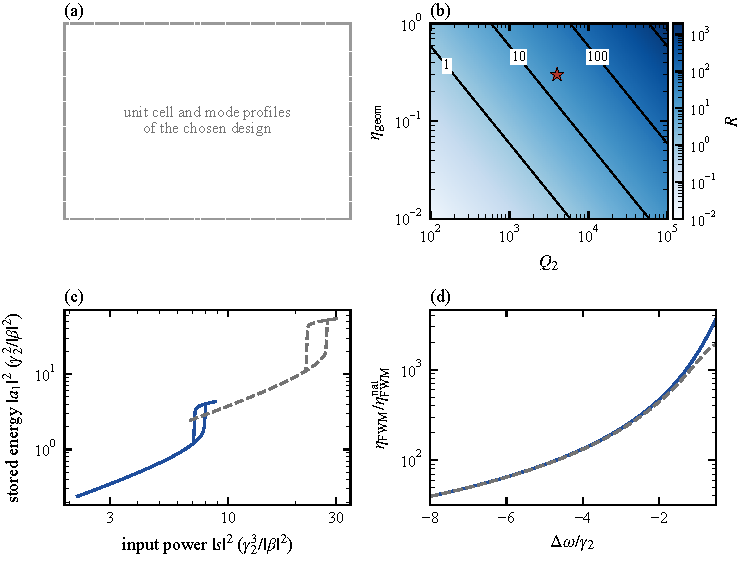
\includegraphics[width=\linewidth]{figures/fig3_double.pdf}
  \caption{Doubly resonant LiNbO$_3$ metasurface.
    (a)~Unit cell with the pump and second-harmonic mode profiles.
    (b)~$R$ from Eq.~\eqref{eq:R} versus $Q_2$ and $\etag$ at
    $\Dom=2\gamma_2$ (colour scale), with contours at $R=1$, 10 and 100; the
    star marks $Q_2=4000$, $\etag=0.3$.
    (c)~Stored pump energy versus input power for increasing and
    decreasing sweeps of Eqs.~\eqref{eq:cmt1} and \eqref{eq:cmt2}, with
    (solid) and without (dashed) the second-harmonic mode, for
    $N_1=N_2=\tfrac12$, $\Dom=-2\gamma_2$, $\gamma_1=\gamma_2$,
    $\gamma_1^{\mathrm e}=\gamma_1/2$, $\alpha_3$ chosen for $R=20$, and in
    each case a pump detuning 1.3 times the minimum for bistability (a cold
    mismatch of $2.4\gamma_2$ in the cascaded case).
    (d)~Ratio of four-wave-mixing efficiencies $\eta_{\mathrm{FWM}}$ with and
    without the second-harmonic mode at equal intracavity pump energy,
    $|\alpha_3+\alpha_{\mathrm{casc}}|^2/\alpha_3^2$ (solid), and $(1+R)^2$
    with $R$ evaluated at each $\Dom$ (dashed), versus $\Dom/\gamma_2$ for
    $\Dom<0$ and the same $\alpha_3$.}
  \label{fig:double}
\end{figure}

\subsection{Singly resonant metasurface and proposed measurement}\label{sec:single}

Without a pump resonance the pump field in the meta-atom is fixed by the
incident wave.  With $\mathbf e_1$ the linear pump field per unit incident
amplitude, the elimination of Section~\ref{sec:theory} applies with $\f_1$
replaced by $\mathbf e_1$.  The overlap becomes
$\widetilde M=\int\chitwo_{ijk}f^*_{2,i}e_{1,j}e_{1,k}\,d^3r$.  For a
meta-atom much thinner than the wavelength, where $\mathbf e_1$ has a
uniform phase, $R$ takes the form of Eq.~\eqref{eq:R} with $\etag$ replaced
by $\eta^{(1)}$, defined as in Eq.~\eqref{eq:eta} with $\widetilde M$ and
$\mathbf e_1$ in place of $M$ and $\f_1$ [Fig.~\ref{fig:single}(b);
Supplement 1, Section 7].  The
nonlinear phase per unit incident power loses the factor $Q_1^2$ of a pump
resonance, and there is no bistability.  The local pump field and the
native response then change little while $\Dom$ is scanned across the
second-harmonic resonance, which makes this structure suited to measuring
the cascaded susceptibility.
% FOR THE DESIGN (Sedigheh): the chosen design [Fig. 4(a)]: geometry, Q2,
% M-tilde, eta^(1), R at Domega = +-2 gamma2 (recipe in Supplement 1,
% Section 7), the single-pass phase, and the absolute figures of merit and
% detectability budget
\textit{[Design: geometry, $Q_2$, $\widetilde M$, $\eta^{(1)}$, $R$ at
$\Dom=\pm2\gamma_2$ and the single-pass phase; Fig.~\ref{fig:single}(a).]}

The part of the response odd in $\Dom$ would be measured with a
closed-aperture Z-scan [Fig.~\ref{fig:single}(c)] as a function of the pump
wavelength, which moves $2\omega_1$ across $\omega_2$, in analogy with the
angle-tuned measurement in KTP~\cite{desalvo1992}.  The cascaded phase stays
within 8\% of its continuous-wave value for pulses longer than
$1.5/\gamma_2$ (intensity FWHM), about 2.5~ps for $Q_2=4000$ at
1.55~\textmu m [Fig.~\ref{fig:single}(d)].  The beam must be wide enough
that its angular spread stays within the angular bandwidth of the
second-harmonic mode~\cite{overvig2022}.  Near a Mie resonance the native
response alone can change the sign of the effective nonlinear
index~\cite{panov2020}.  That contribution follows the pump response,
so the cascaded part is the component odd in $\Dom$ when the pump
transmission is flat across the scan.  The second-harmonic conversion efficiency of the
same sample, together with the radiative part of $\gamma_2$ and the
collection efficiency, would fix $|\widetilde M|$.

\begin{figure}[htbp]
  \centering
  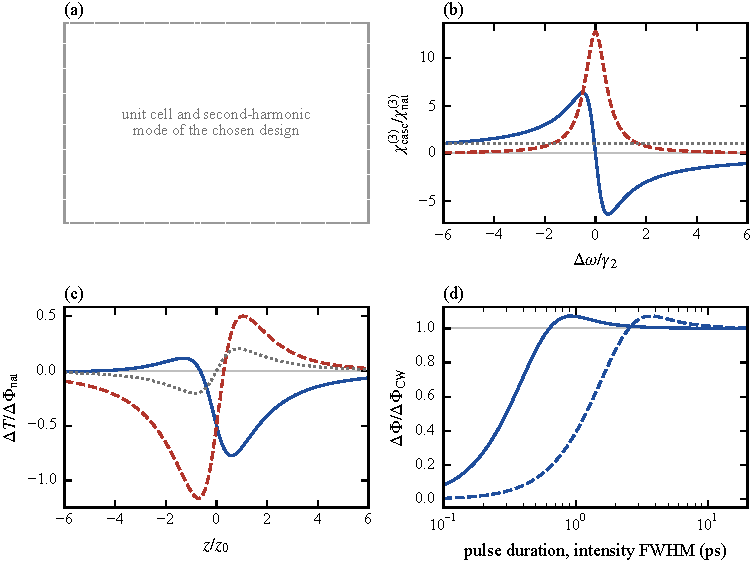
\includegraphics[width=\linewidth]{figures/fig4_single.pdf}
  \caption{Singly resonant LiNbO$_3$ metasurface.
    (a)~Unit cell and second-harmonic mode profile.
    (b)~Real (solid) and imaginary (dashed) parts of $\chicasc/\chinat$
    versus $\Dom/\gamma_2$ for an illustrative value $R=3$ at
    $|\Dom|=2\gamma_2$; the dotted line
    is the native response.
    (c)~Closed-aperture Z-scan transmission change of a thin
    sample~\cite{sheikbahae1990,liu2001}, in units of the native phase
    $\Delta\Phi_{\mathrm{nat}}$, versus the sample position $z$ in units of the
    Rayleigh range $z_0$ ($z<0$ before the focus), for $\Dom=+2\gamma_2$
    (solid), $\Dom=-2\gamma_2$ (dashed) and the native response alone
    (dotted), including the nonlinear absorption of the cascade.
    (d)~Intensity-squared-weighted Z-scan phase of the cascaded response for
    Gaussian pulses, relative to its continuous-wave value, versus the
    intensity FWHM of the pulse at $\Dom=2\gamma_2$, for $Q_2=10^3$ (solid)
    and $4\times10^3$ (dashed), at a pump wavelength of 1.55~\textmu m.
    Horizontal lines mark 0 and 1.}
  \label{fig:single}
\end{figure}


\section{Microring resonators}\label{sec:ring}

In a doubly resonant $\chitwo$ microring [Fig.~\ref{fig:concept}(c)] the
elimination of Section~\ref{sec:theory} reproduces the cavity expression of
Refs.~\cite{cui2022,cui2025}, measured in AlN, with the coupling rate $g$
of the pump and second-harmonic modes in place of the overlap $M$
(Supplement 1, Section 8).  The same rate sets the second-harmonic
efficiency $\eta_{\mathrm{SHG}}=P_{\mathrm{SH}}/P_{\mathrm{in}}^2$ on double
resonance, which is reported for such devices~\cite{lu2019,lu2020,zhao2022}, and
eliminating $g$ expresses the cascaded shift of the pump resonance through
measured quantities.  For a pump locked to its resonance and both modes
critically coupled to the bus waveguide,
\begin{equation}
  \frac{\delta\omega_{\mathrm{casc}}}{\kappa_1}
  =\eta_{\mathrm{SHG}}P_{\mathrm{in}}\,\frac{\kappa_2\Dom}{\Dom^2+\kappa_2^2}
  \label{eq:ringshift}
\end{equation}
when the nonlinear loss is neglected, where $\kappa_n=\gamma_n/2$ are the
half-widths, $P_{\mathrm{in}}$ is the input power and a positive
$\delta\omega_{\mathrm{casc}}$ raises the resonance frequency.  Other
couplings multiply the right-hand side by
$(\kappa_1/2\kappa_1^{\mathrm e})(\kappa_2/2\kappa_2^{\mathrm e})$, where
$\kappa_n^{\mathrm e}$ are the rates of coupling to the bus.
Equation~\eqref{eq:ringshift} contains no overlap, material constant or
mode volume: the second-harmonic power measures the nonlinear loss, and the
ratio $\rho$ of Section~\ref{sec:limits} converts it into the shift.  For
the periodically poled thin-film LiNbO$_3$ ring of Ref.~\cite{lu2020}, with
$\eta_{\mathrm{SHG}}=5\times10^6$\%/W and a coupling factor of 1.6, it
gives 0.09 half-widths, or
17~MHz, against 0.03~MHz for the native response, at 5~\textmu W and
$\Dom=2\gamma_2$ [Fig.~\ref{fig:ring}(b)].  This power lies below the
parametric threshold of the ring and below the power at which
photorefraction lowers the efficiency~\cite{lu2020}; the coupling rate
fitted to the lineshape of the ring would give a shift 4.7 times larger.
To our knowledge, no device has been characterised by
$\eta_{\mathrm{SHG}}$ and the cascaded shift together; measuring the two on
one ring would test Eq.~\eqref{eq:chi3casc} without a fitted parameter.
Thermal and photorefractive shifts~\cite{sun2017,xu2021} are comparable
with or larger than the cascaded shift at these powers, but even in $\Dom$
to leading order.  An electro-optic dither of $\Dom$ with lock-in detection
would separate the odd cascaded part (Supplement 1, Section 8), as the
Z-scan of Section~\ref{sec:single} would in a metasurface.

Relative to the native Kerr response of the same ring, $R$ lies between
$6\times10^2$ and $2.8\times10^3$ for the device of Ref.~\cite{lu2020},
depending on whether $g$ is taken from $\eta_{\mathrm{SHG}}$ or from the
lineshape, and between $4\times10^2$ and $1.8\times10^3$ for a ring with
$Q_1=10^6$ and $Q_2=3\times10^5$.  Without poling it is about 13
[Fig.~\ref{fig:ring}(a)].  In the latter ring the parametric threshold
falls from 9~mW for the native response to 8~\textmu W, below the
bistability threshold of 37~\textmu W (Supplement 1, Section 8).  Because
the sign of the Kerr term follows that of $\Dom$, one ring can provide
either sign for modulation instability and comb
formation~\cite{leo2016,lu2023,tang2024}.

\begin{figure}[htbp]
  \centering
  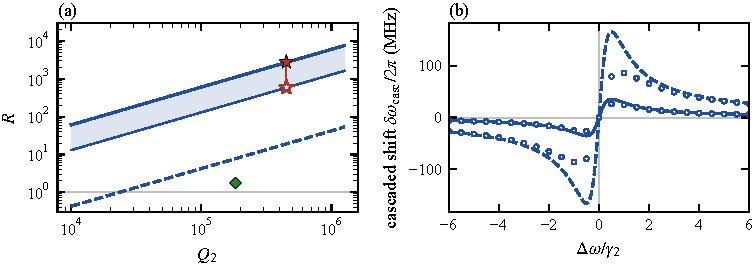
\includegraphics[width=\linewidth]{figures/fig5_ring.pdf}
  \caption{Microrings.
    (a)~$R$ versus $Q_2$ at a cold mismatch of $2\gamma_2$ for a periodically
    poled LiNbO$_3$ ring (design B of Supplement 1, Table S2) with the
    coupling rate scaled from the fitted value of Ref.~\cite{lu2020} (upper
    solid line) or from its measured efficiency (lower solid line), and
    without poling (design C, dashed), with intrinsic $Q_2$ twice the loaded
    value.  Stars: the device of Ref.~\cite{lu2020} for the two coupling
    rates.  Diamond: the AlN ring of Ref.~\cite{cui2025}, from its measured
    tuning of the self-phase modulation scaled to $\Dom=2\gamma_2$.  The
    horizontal line marks $R=1$.
    (b)~Cascaded shift of the pump resonance of the device of
    Ref.~\cite{lu2020} versus $\Dom$ at 5~\textmu W input, from
    Eq.~\eqref{eq:ringshift} with the coupling factor of the device and the
    measured efficiency (solid) and with
    the efficiency implied by the fitted coupling rate (dashed).  Circles:
    steady state with the pump locked to the shifted resonance, including
    the nonlinear loss.  The pump half-width is
    $\kappa_1/2\pi=178$~MHz.}
  \label{fig:ring}
\end{figure}


\section{Discussion and conclusion}\label{sec:discussion}

\begin{table}[htbp]
  \caption{\bf Cascaded Kerr Response on Five Platforms ($R$ at $\Dom=2\gamma_2$)}
  \label{tab:platforms}
  \centering
  \small
  \setlength{\tabcolsep}{4pt}
  \begin{tabular}{llcccc}
    \hline
    Platform & Set by & $Q_2$ & $R$ & Bandwidth & CW threshold \\
    \hline
    Bulk LiNbO$_3$ & $\Delta k$ & -- & $\approx2$ & $>10$~THz & bistability \\
    Doubly resonant metasurface & $\Dom$ & $4\times10^3$ & $\approx20$ & $\approx0.1$~THz & bistability \\
    Singly resonant metasurface & $\Dom$ & design & design & design & none \\
    AlN microring~\cite{cui2025} & $\Dom$ & $1.8\times10^5$ & $1.7$\,$^a$ & $\approx0.3$~GHz & -- \\
    Poled LiNbO$_3$ microring & $\Dom$ & $3\times10^5$ & $4\times10^2$--$1.8\times10^3$ & $\approx0.2$~GHz & 8~\textmu W, parametric \\
    \hline
  \end{tabular}

  \smallskip
  \footnotesize Bandwidth: response bandwidth for the bulk crystal and the
  linewidth of the narrower resonance otherwise, which is the
  second-harmonic mode for the metasurface and the pump mode for the rings.
  $R$ assumes $\etag=0.3$ for the doubly resonant metasurface and spans the
  two values of the coupling rate for the microring.  CW threshold: the
  continuous-wave instability that appears first, observed for bulk
  LiNbO$_3$ in a cavity resonant at the pump~\cite{white1996} and predicted
  for the metasurface.  For the microring the entry gives the input power at
  the parametric threshold; its bistability threshold is 37~\textmu W.
  $^a$From the measured tuning of the self-phase modulation, $-2.7$ to
  $+4.7$ times its calculated native value at the extrema of the tuning
  curve, $|\Dom|=\gamma_2/2$~\cite{cui2025}, scaled to $\Dom=2\gamma_2$.
\end{table}

A detuned second-harmonic resonance gives a cascaded Kerr nonlinearity of
either sign, whose strength is set by $Q_2$, $\Dom$ and $\etag$ and which
depends on the host only through $F$.  In LiNbO$_3$ we estimate it at about 20 times the
native response in a doubly resonant metasurface and several hundred to a
few thousand times in a poled microring (Table~\ref{tab:platforms}).
Because Eq.~\eqref{eq:sumrule} bounds the product of strength and
bandwidth, a larger $R$ comes with a narrower bandwidth.  The
second-harmonic linewidth, which sets the response time of the cascade, is
about 1~GHz in the ring and 0.1~THz in the metasurface, and bulk cascading,
which is weaker, extends beyond 10~THz.  Of the three, the metasurface is
the only sub-micrometre layer addressed from free space, and its response
is fast enough for picosecond pulses.
% FOR THE DESIGN (Sedigheh): outlook on applications (picosecond all-optical
% modulation with a sign set by Domega, thin films with cancelled or reversed
% Kerr response) once the design and its absolute figures of merit are known.
Engineered second-order media would raise $R$ through
$|\chitwo|^2$, as in coupled quantum wells with an interband $\chitwo$ above
$10^3$~pm/V~\cite{ramesh2026} and quantum-well
metasurfaces~\cite{fathi2026}, provided the native response and the
absorption near the band edge~\cite{sheikbahae1991}, which also limit the
second harmonic, stay small.

\begin{backmatter}
\bmsection{Funding}

\bmsection{Disclosures}
The authors declare no conflicts of interest.

\bmsection{Data availability}
Write here something.

\bmsection{Supplemental document}
See Supplement for supporting content.
\end{backmatter}

\bibliography{refs}

\end{document}
